
\section{Contrôle du Robot} 

Dans cette section nous discuterons les choix d'architecture, la mise en oeuvre des packages ROS que nous ferons tourner sur le robot et les résultats obtenus. Les indications de comment éxecuter le code se trouvent dans la subsection \ref{result}

\subsection{Choix d'architecture}

Nous avons choisi de travailler avec ROS (Robot Operating System), un middleware de robotique conçu pour aider à abstraire les détails de hardware, pour qu'on puisse accéder aux fonctionnalités de haut niveau des robots d'une forme simple. Le fonctionnement de ROS est basé sur l'exposition des ressources du système parmi des \textbf{noeuds} qui peuvent se communiquer entre eux parmi des \textbf{messages} qui sont envoyés à des \textbf{topiques}, entités responsables de recevoir les messages des noeuds appelés \textbf{publishers} et les envoyer aux noeuds appelés \textbf{subscribers}. Les ressources incluent les moteurs et les capteurs, bien que les ressources de computation. Avec ces concepts basiques de ROS, nous allons présenter l'architecture du système, qui est résumé dans la figure suivante.

\begin{figure}[!h]
  \centering
	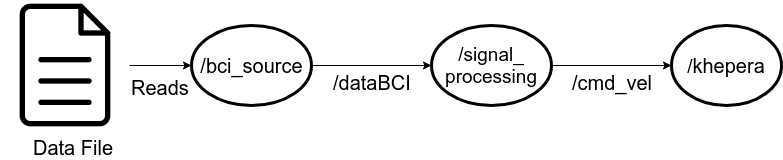
\includegraphics[scale=0.40]{images/ArchiDiagram.png}
	\caption{Diagramme conceptuel du système, où les ellipses représentent des noeuds et les flèches représentent des topiques (sauf la flèche 'Reads')}
	\label{fig:archDiag}
\end{figure}


Pour simuler l'acquisition en temps réel des signaux BCI on a décidé de faire tourner un noeud appelé /bci\_source qui au moment de l'initialisation lit un fichier contenant un vrai signal pré-enregistré (fourni au début du projet) et après il rentre dans une boucle d'exécution, publiant un message sur le topique /dataBCI à la fois. Chaque message s'agit d'un float qui correspond à un échantillon du signal. Pour garantir que la simulation soit bien adapté, ce noeud tourne à une fréquence égale à la fréquence d'échantillonage du signal, dans ce cas 256 Hz. Le fichier contient aussi les labels des commandes correspondantes qui sont affichés dans l'écran lors de l'exécution du noeud pour que l'utilisateur puisse avoir au moins une idée du comportement du système. Le fichier correspondant à ce noeud se trouve sur '/projectRoot/ros\_ws/bci\_robot/scripts/bci\_source.py'.

Le noeud /signal\_processing est un \textit{subscriber} du topique /dataBCI, il reçoit des échantillons à 256 Hz. Différemment de l'approche qu'on a pu tenir dans les sections précédentes, ici nous sommes obligés de traiter les échantillons tant qu'ils viennent, et pas dans un coup du début à la fin. Après quelques discussions dans le groupe et avec les encadrants nous avons décidé filtrer le signal tant qu'il vient et stocker les estimations de puissance en chaque fréquence centrale dans une espèce de buffer de taille fixe, et une fois que ce buffer est rempli nous publions un message de commande au robot correspondant à une moyenne des signaux dans ce buffer pour chaque fréquence. Les calculs faites lors du traitement du signal sont les mêmes que ceux décrits précédemment, c'est à dire, on passe le signal \(x[n]\) pour trois filtres passe-bandes de fréquences centrales 7.5, 11 et 13.5 Hz, obtenant ainsi trois signaux \(y_i[n]\). À partir de ces signaux on estime la puissance présente en chaque bande de fréquence, obtenant trois signaux \(z_i[n]\), et ces z seront, donc, stockés dans le buffer. La stratégie pour choisir une commande à partir de ces signaux \(z_i[n]\) a été déjà exploré dans la section précédente, mais nous y reviendrons dans la subsection suivante. Finalement, après avoir choisi la bonne commande le noeud /signal\_processing publie un message du type \textit{Twist} au robot parmi le topique /cmd\_vel. La fréquence de publication de ce noeud est directement lié à celle du noeud d'avant, et si \(f_e\) est la fréquence d'échantillonage du signal original et \(N\) la taille du buffer, la fréquence de publication sera de \(f_e/N\). Le fichier correspondant à ce noeud se trouve sur '/projectRoot/ros\_ws/bci\_robot/scripts/signal\_pro.py'.

Finalement, le noeud du robot khepera sera un \textit{subscriber} du topique /cmd\_vel, d'où il va recevoir les consignes de vitesse correspondantes. Passons maintenant aux détails de mise en oeuvre.

\subsection{Mise en oeuvre du système et résultats} \label{result}

Nous avons choisi python comme langage pour implémenter ces deux noeuds, dont les fichiers se trouvent dans le répertoire '/projectRoot/ros\_ws/bci\_robot/scripts'. Pour faciliter le débugage et permettre de tester le programme même sans le robot, on a ajouté une option pour envoyer les messages à un noeud turtlesim au lieu du khepera. On décrira pas à pas comment faire tourner le système tant que nous expliquons les détails de sa mise en oeuvre.

D'abord, il faut \textit{builder} les packages ros. On va faire référence à la racine du projet comme \textbf{projet}, donc allez sur projet/ros\_ws et tapez:
\begin{lstlisting}[language=bash]
  $ catkin_make
  $ source devel/setup.bash
\end{lstlisting}

Ouvrez un terminal et faites tourner le roscore:

\begin{lstlisting}[language=bash]
  $ roscore
\end{lstlisting}

Maintenant passons au noeud /bci\_source. Si vous allez sur \textit{projet/obj} vous verrez tous les enregistrements qui peuvent être utilisés avec ce noeud. Alors, tapez: 
\begin{lstlisting}[language=bash]
  $ rosrun bci_robot bci_source.py [path_to_file]
\end{lstlisting}
Où [path\_to\_file] c'est le chemin complet pour un de ces fichiers sur projet/obj. Ouvrons 'herve002\_labeled.txt' par example:

\begin{figure}[!h]
  \centering
	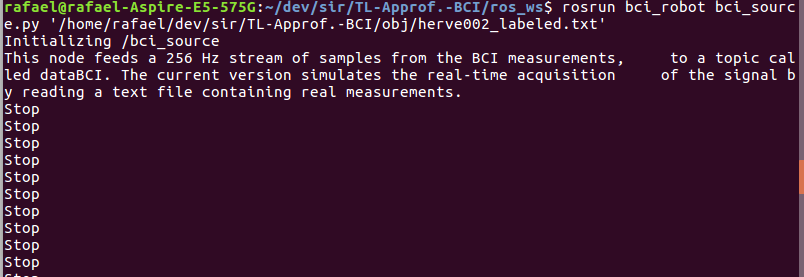
\includegraphics[scale=0.50]{bci1.png}
	\caption{Fonctionnement du noeud /bci\_source}
	\label{fig:bci1}
\end{figure}

Vous verrez que ce noeud est en train de publier des messages sur le topique /dataBCI, tapez:
\begin{lstlisting}[language=bash]
  $ rostopic echo /dataBCI
\end{lstlisting}

Et vous verrez quelque chose similaire à ce qu'on a dans la figure \ref{fig:bci2}

\begin{figure}[!h]
  \centering
	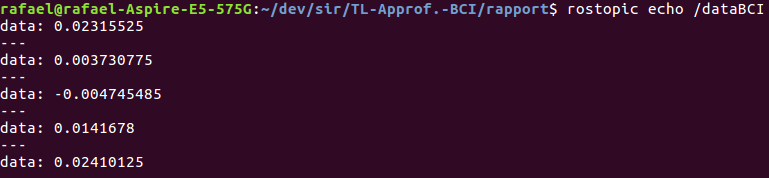
\includegraphics[scale=0.50]{bci2.png}
	\caption{Publication des échantillons sur /dataBCI}
	\label{fig:bci2}
\end{figure}

Le noeud est un simple publisher et il continue à publier les échantillons jusqu'à la fin du fichier, et là il s'arrête e termine le programme.

Passons au noeud /signal\_processing. Ouvrez un nouveau terminal et tapez:

\begin{lstlisting}[language=bash]
  $ rosrun bci_robot signal_pro.py turtle
\end{lstlisting}

Ici nous utilisons l'option 'turtle', parce que nous publierons les commandes dans le topique du turtlesim, pour le faire publier sur le topique du khepera il suffit de changer 'turtle' pour 'khepera'. Si jamais votre noeud /bci\_source a fini de publier tout le signal et a affiché 'Finished publishing the data from file' relancez-le. Vous aurez quelque chose comme la figure \ref{fig:bci3}

\begin{figure}[!h]
  \centering
	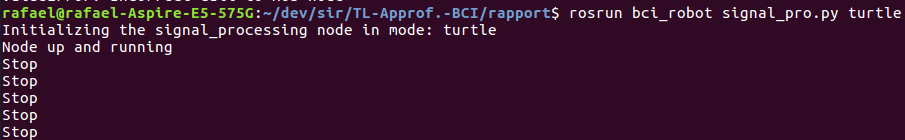
\includegraphics[scale=0.50]{bci3.png}
	\caption{Initialisation et affichage du noeud /signal\_processing.}
	\label{fig:bci3}
\end{figure}

Différemment du /bci\_source, ce noeud est implémenté comme une classe appelé \textbf{Signal\_processer} (l'autre est défini comme un e simple fonction), afin de stocker les paramètres et avoir accès facile à ces variables. L'initialisation de la classe est faite de façon paramétrable, où on peut choisir la taille du buffer, les vitesses du robot, le mode d'opération, bien que mettre en place les paramètres optimales obtenus auparavant. Ce noeud est aussi un subscriber ainsi qu'un publisher. Il possède une fonction \textbf{callback\_data\_listen()} (cf. signal\_pro.py) qui est appelé à chaque fois qu'il reçoit un message du topique /dataBCI, et qui traite les échantillons, un la fois, tant qu'ils arrivent, et ainsi cette fonction est appelé à une fréquence de 256 Hz. Elle a un comportement cyclique dans lequel elle va remplir le buffer à chaque nouvel appel en bougeant un compteur de position en position, mais quand le buffer est plein, cette fonction fait appel à une autre fonction \textbf{callback\_pub()} et mets le compteur à zéro. Cette fonction callback\_pub, par contre, correspond au côté publisher du noeud, et donc elle va utiliser toute l'information présente dans le buffer pour choisir la bonne commande e la publier sur le topique choisi. La fonction responsable pour trouver cette bonne commande est \textbf{get\_command()}. D'abord cette fonction doit utiliser toute l'information dans le buffer, et la façon la plus simple de le faire c'est de faire la moyenne de chacun des 3 signaux dans le buffer. Une approche plus intéressante serait de normaliser ce buffer par une fenêtre (Hamming, Blackman etc) pour diminuer l'effet de bord introduit par la fenêtre rectangulaire du buffer, mais faire juste la moyenne nous rends déjà des résultats intéressants. Après, comme décrit précédemment, la fonction va utiliser 3 seuils obtenues parmi une optimisation en grid search, et va diviser chacun des 3 signaux par le seuil correspondent. De cette façon, quand toutes les signaux sont inférieurs à 1, tous les signaux originales sont en dessous des seuils et ainsi on choisira la commande 'Rien'. L'effet de normaliser les 3 signaux par ces seuils c'est que, une fois que au moins un de ces signaux est au dessus du seuil, il suffit juste de choisir entre eux le plus grand et appliquer la commande correspondante. Les vitesses appliqués par les commandes sont définis par les paramètres de la classe Signal\_processer.   

Pour voir le fonctionnement des deux noeuds ensemble, faites-les tourner après lancer le noeud turtlesim, en tapant:
\begin{lstlisting}[language=bash]
  $ rosrun turtlesim turtlesim_node
\end{lstlisting}

ou en lançant le noeud du khepera.
